\section{Why hit times fail}\label{sec:hitsfail}
\sectionstate{partial}{\texttt{WAVEFORM\_FIRST\_THREADING.md} \S3 (det3); \texttt{THREADING\_DISPLAYS\_2026-07-28.md}; fleet extension R1}
\intent{Each per-strip hit time is an aggregate of the strip's own charge and delayed copies of its neighbours'
($\sim$29\,\% at $\tau\approx47$\,ns to $\pm1$). The drift-time ladder is compressed by 20--30\,\%, reads $\sim$4\textdegree{}
too steep, and the cluster fans away from the track with depth, for rising-edge, CFD and matched-filter times alike.}
\analysis{R1}{hit tiers on r06 for all five chambers}
\begin{figure}[t]
  \centering
  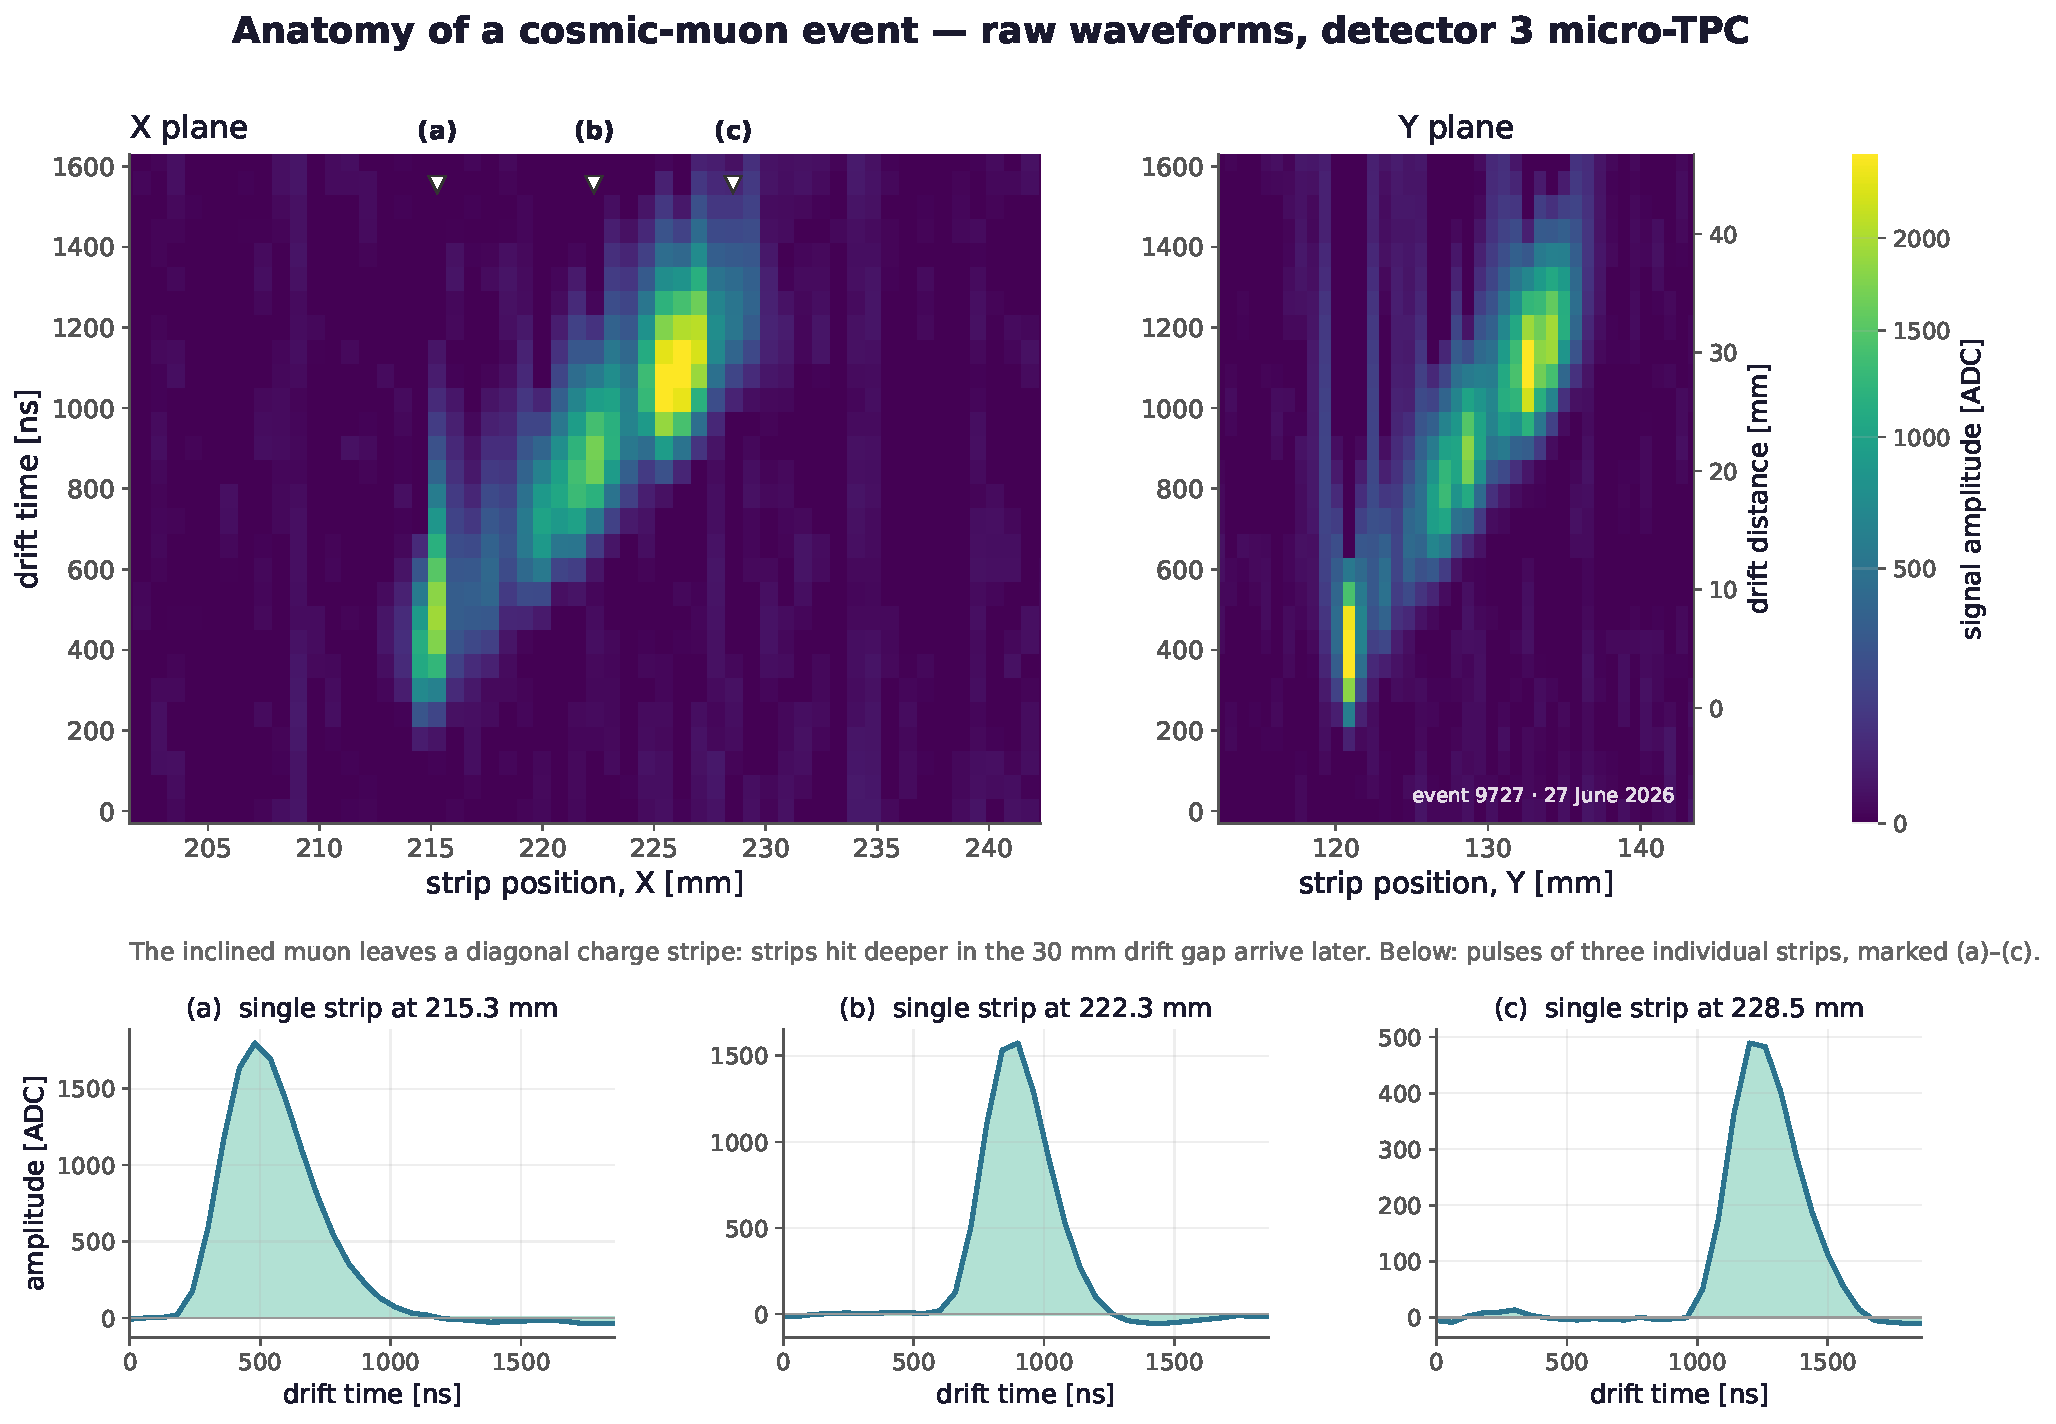
\includegraphics[width=0.85\linewidth]{event_waveforms}
  \caption{\tbw{The strip waveforms of one cosmic track.}}
  \label{fig:event_waveforms}
\end{figure}
\begin{figure}[t]
  \centering
  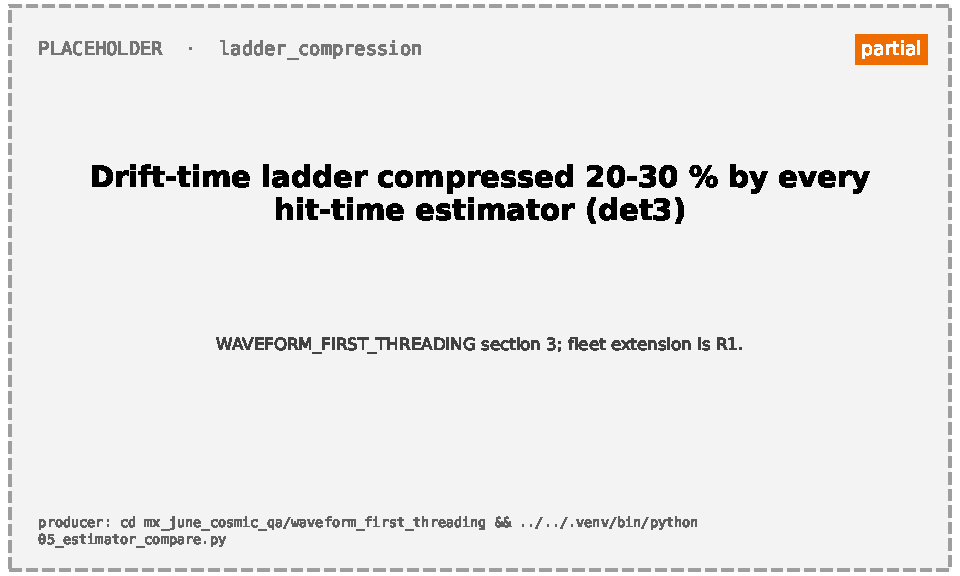
\includegraphics[width=0.8\linewidth]{ladder_compression}
  \caption{\tbw{The drift-time ladder from hit times, per estimator, against the reference.}}
  \label{fig:ladder_compression}
\end{figure}
